\documentclass[a4paper]{article}

\usepackage[utf8]{inputenc}
\usepackage[dutch]{babel}
\usepackage{fancyhdr} %Why the hell does the KU Leuven not have it's own latex header package but the KULAK does?
\usepackage{amsmath}
\usepackage{graphicx}
\usepackage[space]{grffile}
\usepackage{authblk}
\graphicspath{{D:/Jonas/Google Drive/KULeuven3/NumeriekeModelleringBenadering/Practicum/images/}}

\pagestyle{plain}
\title{Numerieke Modellering \& Benadering Practicum}
\author{Dennis Debree}
\author{Jonas Bertels}
\affil{KU Leuven Departement Computerwetenschappen}


\begin{document}
\maketitle
\section{Bivariate Veelterm Benadering}
\subsection{Inleiding}
Voor het vak numerieke modellering en benadering aan de KU Leuven werd de opdracht gegeven een bivariate veelterm benadering te implementeren in MATLAB. Deze benadering werd dan gebruikt om enkele 2 dimensionale oppervlakken te benaderen. Dit verslag geeft een visueel overzicht van de benaderingen en hun oppervlak en van de nauwkeurigheid van de benadering afhankelijk van de graad van de benaderende veelterm.
\subsection{De basisfunctie}
\begin{verbatim}
function C = kkb(x, y, F, m, n)
Afull = fliplr(vander(x)); % we do it this way because it saves us from
Bfull = fliplr(vander(y)); % calculating the inverse twice
C = reshape(kron(Afull(:, 1:m),Bfull(:, 1:n))\F(:), [n,m]);
end
\end{verbatim}
Deze functie creëert eerst de A en B Vandermonde matrices om hieruit de x en y waarden te halen. Daarna wordt uit deze A en B matrices de F matrix berekent door eerst de graad van de A en B matrices te verkorten tot m en n en hierna C te bereken door de formule $C = B^{+}F(A^{+})^{T}$ om te zetten. Dit gebeurt als volgt:
\begin{equation}
C = B^{+}F(A^{+})^{T} \label{solution}
\end{equation}
We weten ook dat:
\begin{equation}
(A\otimes B)^{+} = A^{+} \otimes B^{+} \label{distribution}\\
\end{equation}
\begin{equation}
(A\otimes B)\text{vec}(F) = \text{vec}(BFA^{T}) \label{transformation}
\end{equation}
Uit \eqref{distribution} en \eqref{transformation} kunnen we dan afleiden dat
\begin{equation}
\text{vec}(C) = \text{vec}(B^{+}F(A^{+})^{T}) = (A^{+}\otimes B^{+})\text{vec}(F) = (A\otimes B)^{+}\text{vec}(F) \label{singleInverse}\\
\end{equation}
De reden dat oorspronkelijk \eqref{singleInverse} werd gebruikt in plaats van \eqref{solution} was dat we dachten dat \eqref{singleInverse} ons toeliet om slechts 1 inverse matrix uit te rekenen in plaats van 2 en zo de hoeveelheid benodigd werk doet dalen. Dit was natuurlijk fout omdat $A\otimes B$ dimensies heeft die het product zijn van de A en B matrices apart. Toen de functiebenadering van de Etna moest gegenereerd worden bleek al snel dat het gebruik van \eqref{singleInverse} helemaal geen optimalisatie was in termen van geheugen. Het Kronecker product zorgde er namelijk voor dat matrices zo groot werden dat ze niet meer in het geheugen pasten, en dat bij kleinere waarden van $m$ en $n$ het verschillende minuten duurde voordat de matrix gegenereerd werd (dit is logisch want bij een $m = n = 25$ is $\dim(A) = 1425\times25$ en $\dim(B) = 1425\times25$ waardoor het Kronecker product een dimensie van $2030625\times625$ had).

\subsection{2 functiebenaderingen}
\begin{figure}
\caption{Functiebenadering van $\sin ((2x - 1)^{2} + 2y)$}
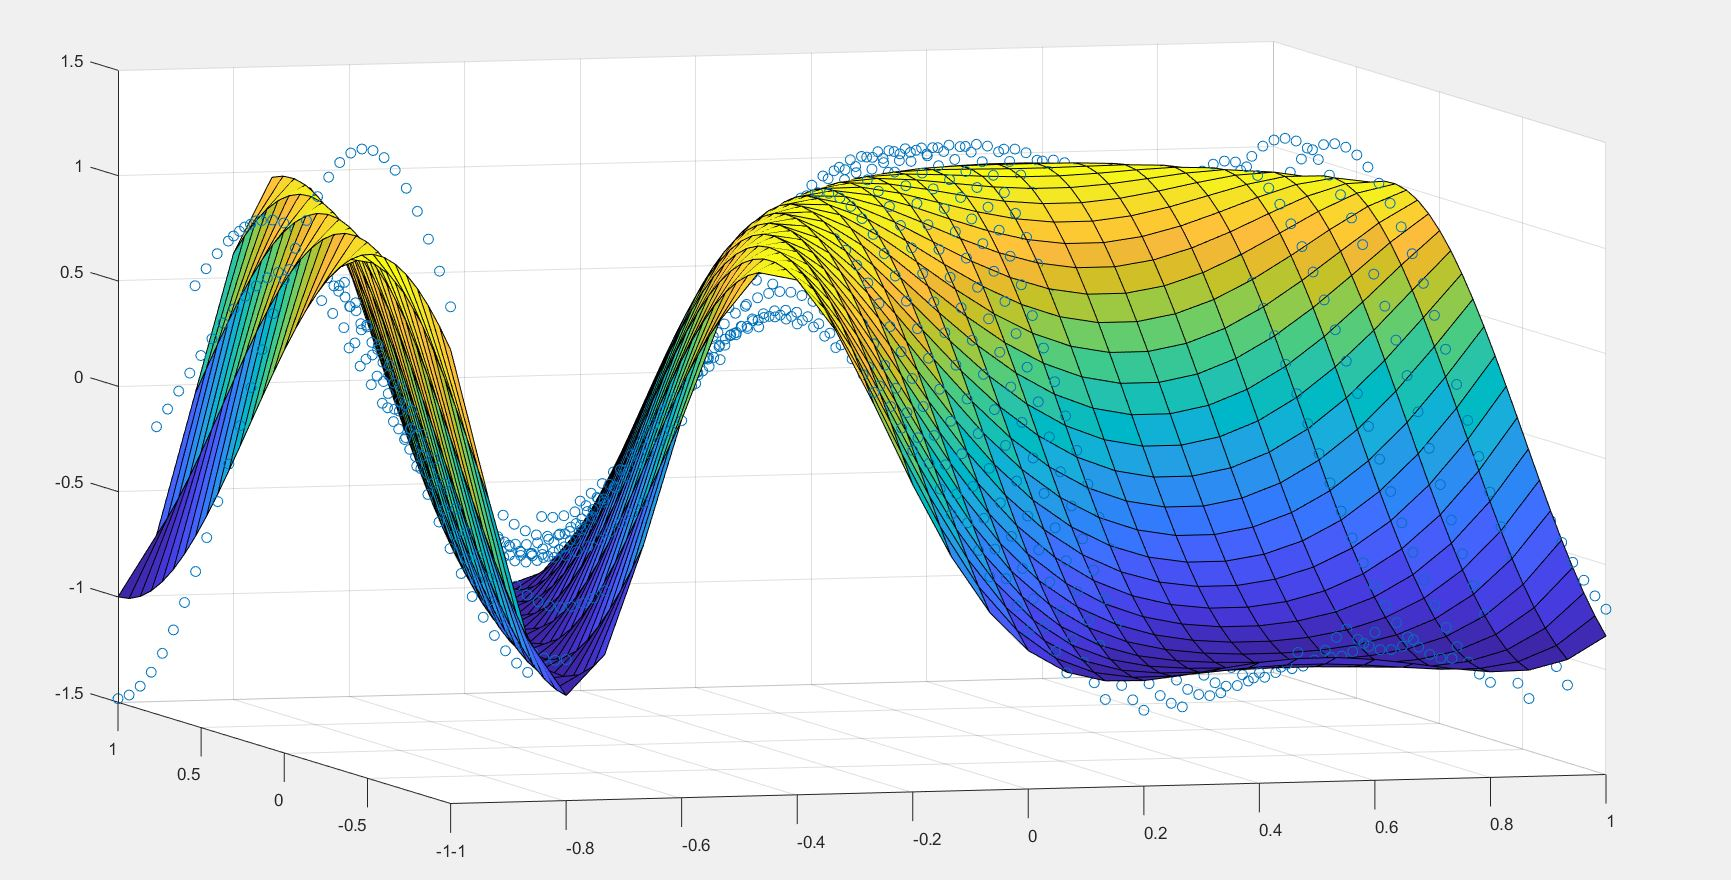
\includegraphics[width=\textwidth, height=0.3\textheight]{Excercise12Sin.JPG}
\end{figure}
\begin{figure}
\caption{Functiebenadering van de membraan functie}
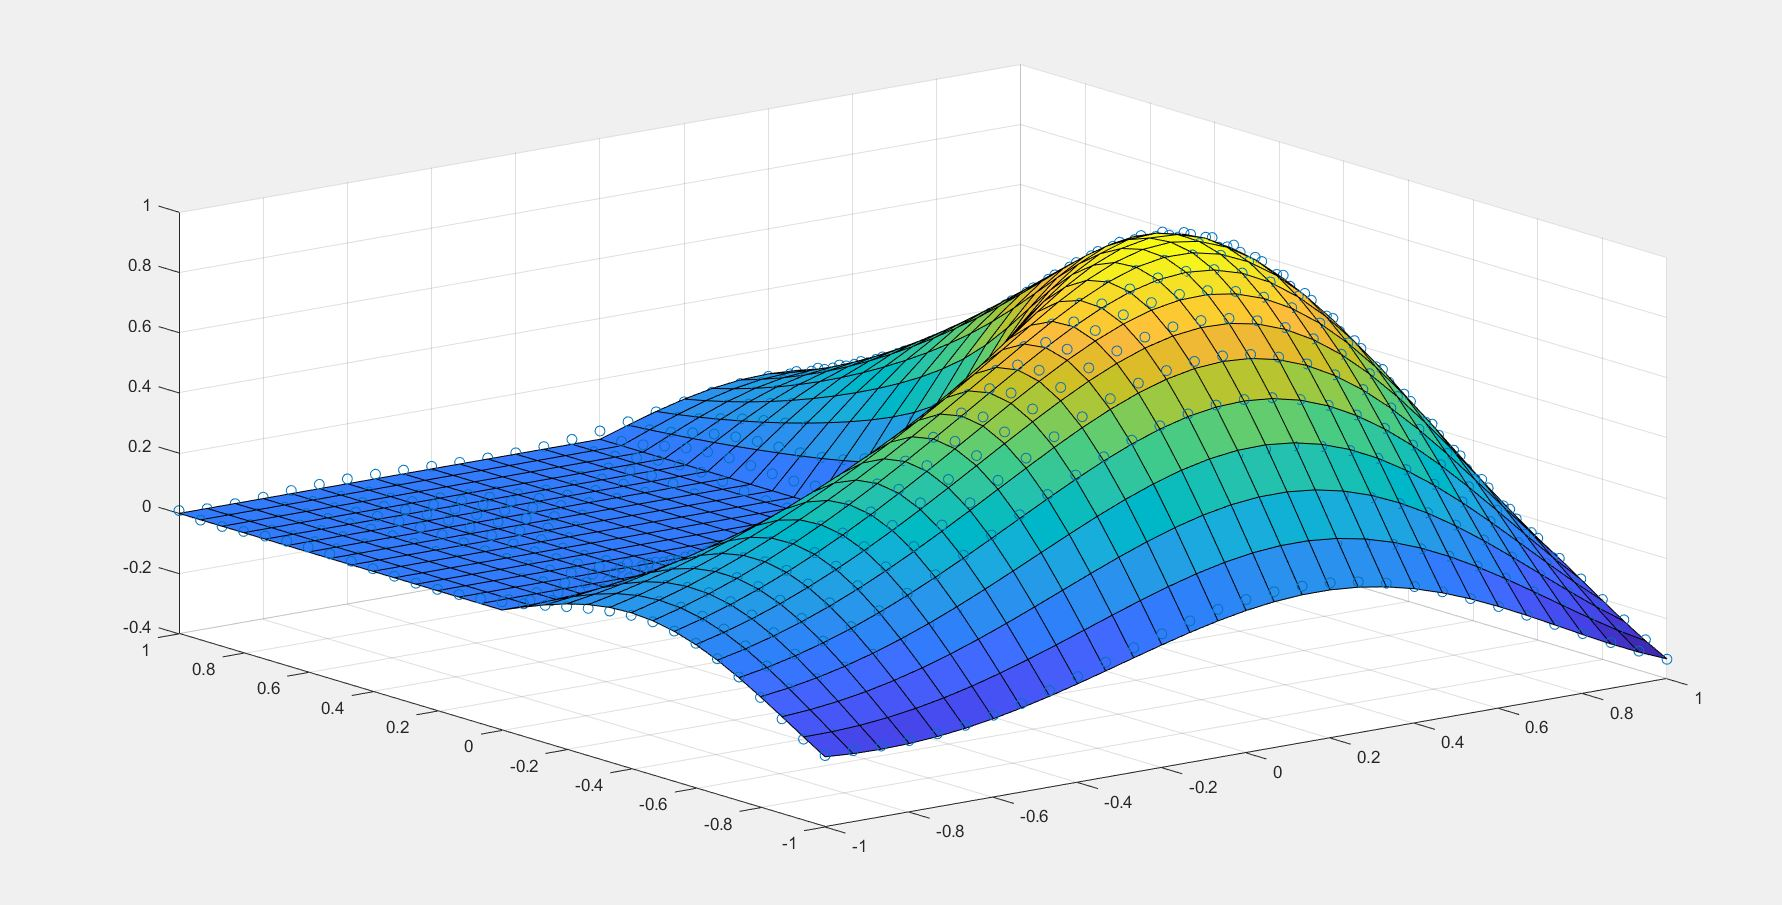
\includegraphics[width=\textwidth, height=0.3\textheight]{Excercise12Membrane.JPG}
\end{figure}
We gebruiken nu de kkbtest functie om enkele 2-D oppervlakken te benaderen. De gegeven functie polyval laat ons toe aan de hand van het resultaat van onze kkb-functie de benaderde waarden voor x en y te evalueren. Op de 2 figuren is de functie voorgesteld als een oppervlak en de benaderde waarden als punten (de blauwe cirkels) die boven of onder dit oppervlak verschijnen.

\subsection{De kostfunctie afhankelijk van de graad van de benaderende veelterm}
De volgende stap is het effect bepalen van de graad van de benaderende veelterm op de nauwkeurigheid van de benadering. Om dit te doen gebruikten we de volgende formule: $\sum_{i=1}^{M}\sum_{j=1}^{N}(f_{ij}-z(x_{i},y_{j}))^{2}$.
\begin{figure}
\caption{Cost Functie als functie van n=m}
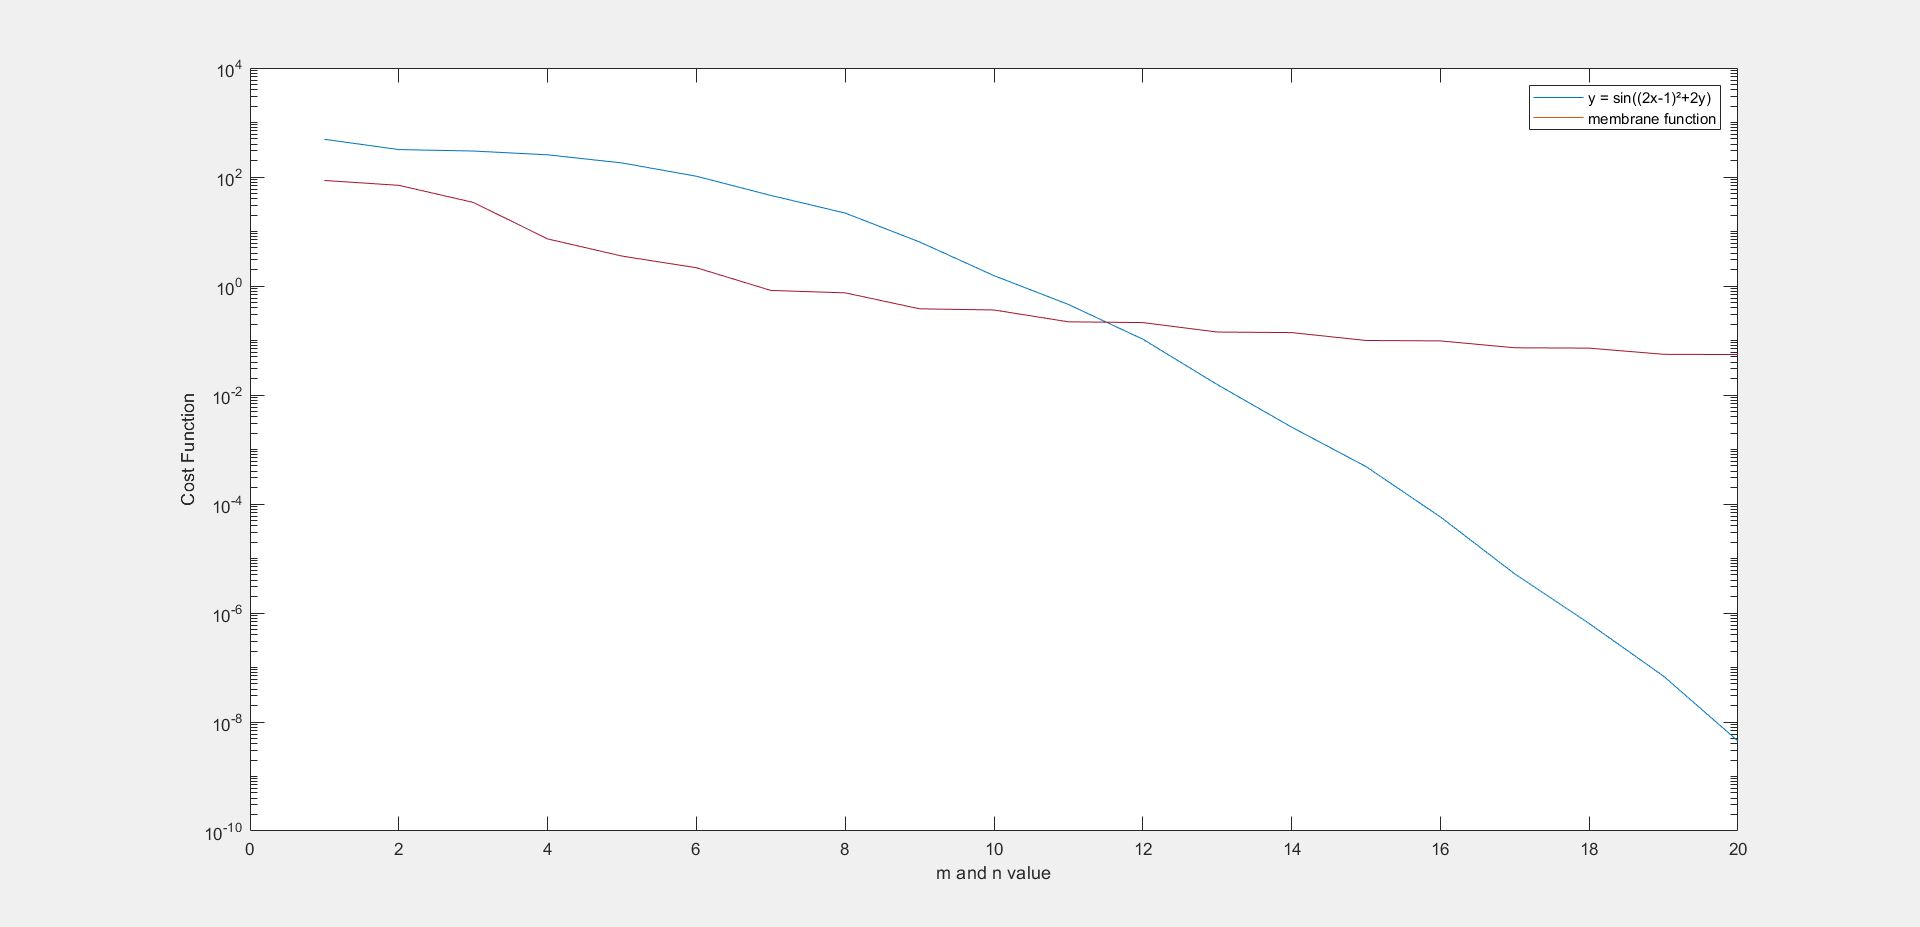
\includegraphics[width=\textwidth, height=0.3\textheight]{Excercise13.JPG}
\end{figure}
\subsection{Veeltermbenadering Etna}
De veeltermbenadering van de Etna werd op praktisch dezelfde manier geïmplementeerd als de functiebenaderingen in oefening 1.2. Zoals al eerder vermeld kwam het door deze functiebenadering dat we begrepen dat onze oorspronkelijk implementatie van kkb niet optimaal was.
\begin{figure}
\caption{De Etna volgens  ASTER Global Digital Elevation Map}
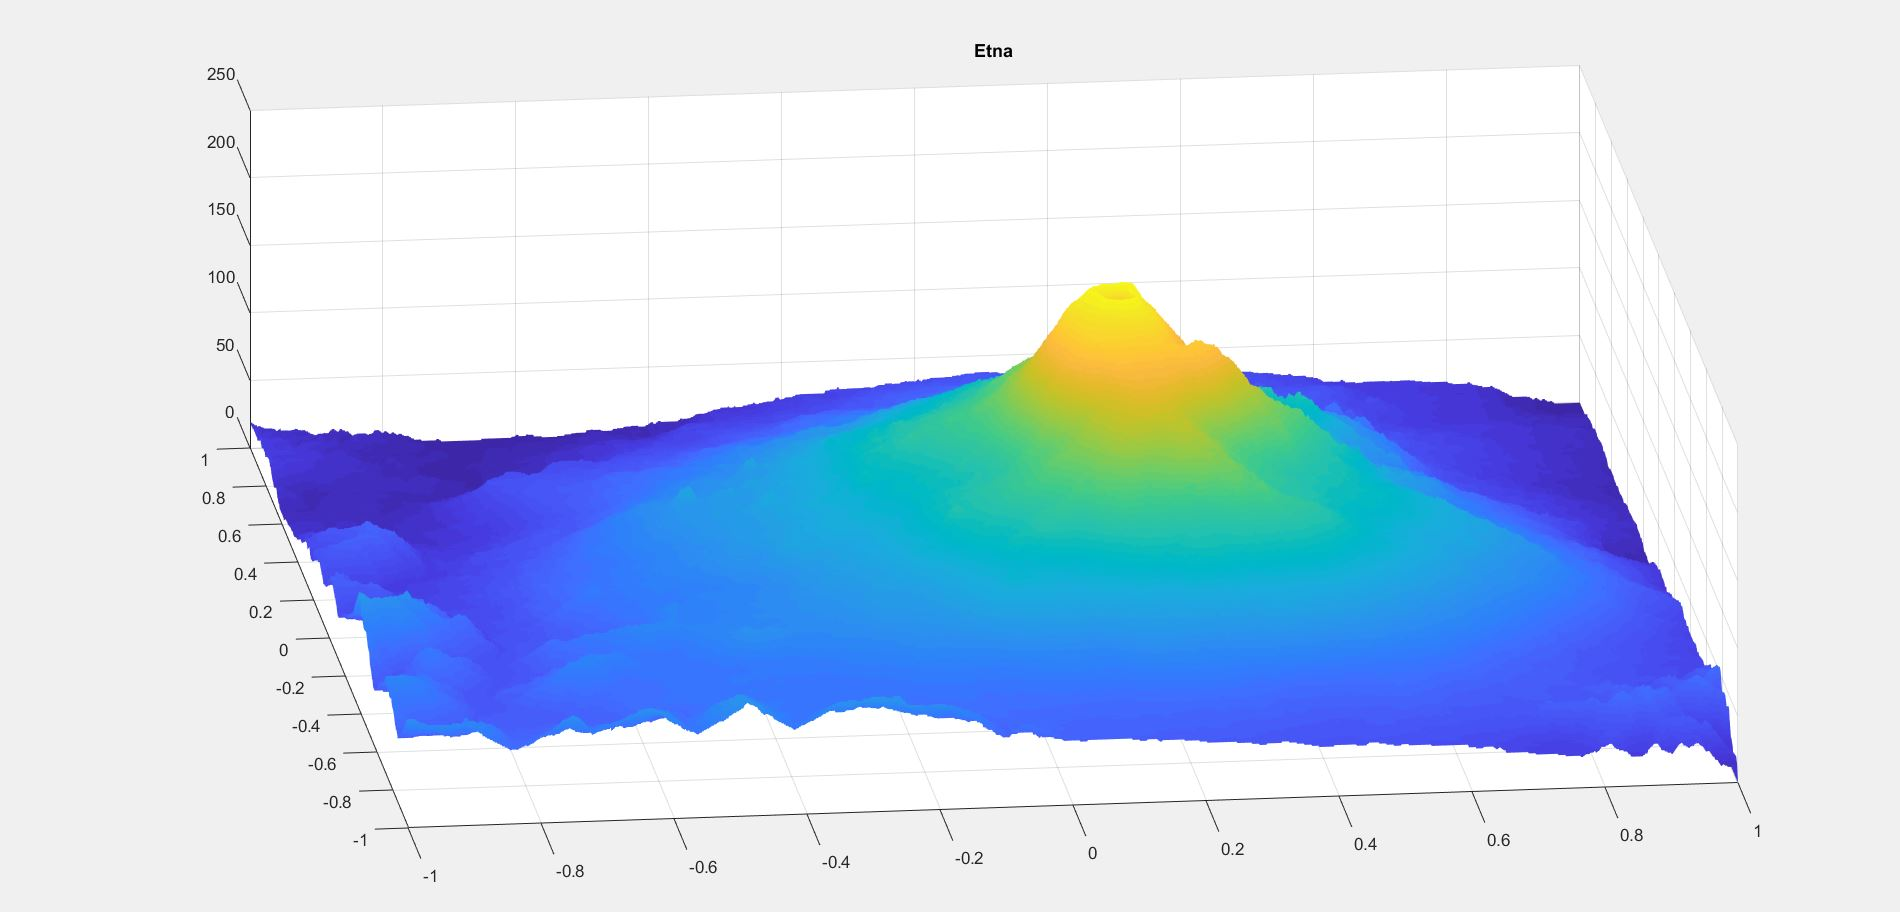
\includegraphics[width=\textwidth, height=0.3\textheight]{Excercise14Etna.JPG}
\end{figure}
\begin{figure}
\caption{Functiebenadering van de Etna met $m = n = 25$}
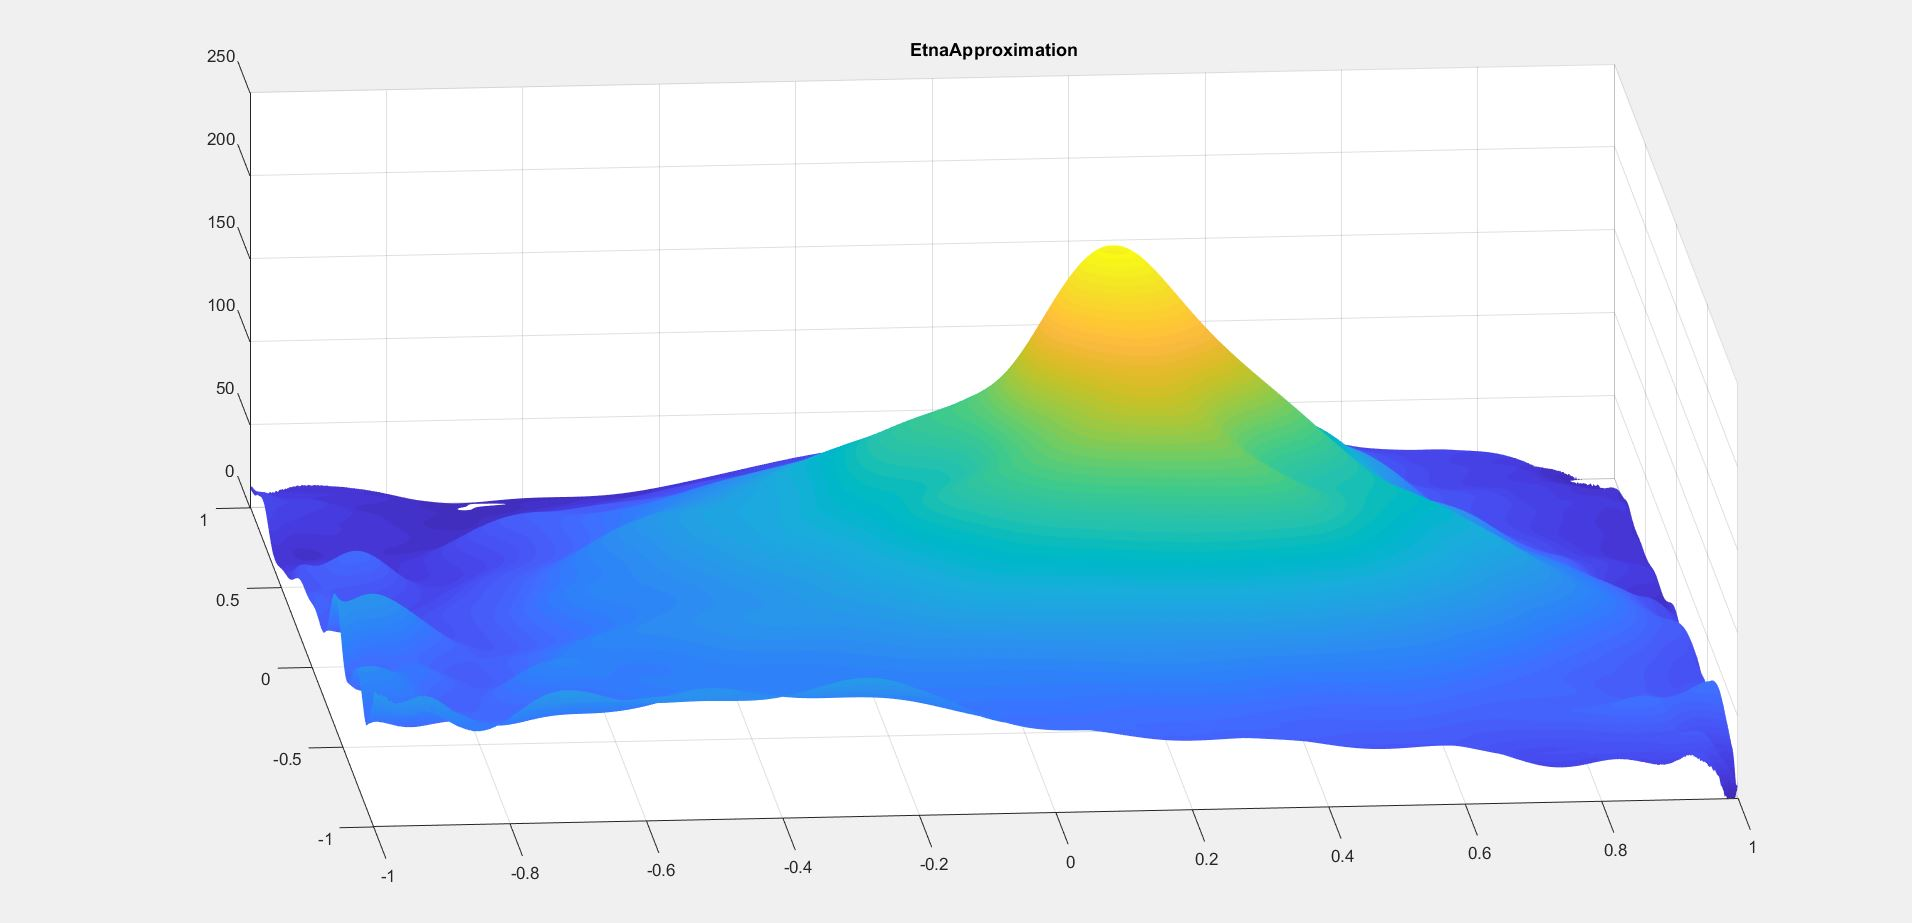
\includegraphics[width=\textwidth, height=0.3\textheight]{Excercise14EtnaBenadering.JPG}
\end{figure}

\end{document}